\chapter{Estado del arte}
En todo proceso de investigación y desarrollo de software, es importante dedicar un tiempo a examinar en que punto se encuentra la investigación en dicho campo. Por tanto, antes de empezar a diseñar nuestra solución nos dedicaremos al análisis de diversas plataformas y editores que resuelven problemas similares al que nos ocupa.

Dedicaremos este capítulo al análisis de diversas plataformas online y editores WYSIWYG. Nos centraremos principalmente en Wikipedia, Stackoverflow y algunos editores como YUI Rich Text Editor~\cite{YUIEditor:yuieditor}, NicEdit~\cite{NicEdit:nicedit}, CKEditor~\cite{CKEditor:ckeditor}, TinyMCE~\cite{TinyMCE:tinymce} y openWYSIWYG~\cite{openWYSIWYG:openwysiwyg}.

\section{Plataformas}
\subsection{Wikipedia}

Wikipedia usa un editor WYSIWYM (What You See IS What You Mean) bastante simple, usando solo las características que la plataforma necesita. Este tipo de editores se caracteriza por una total separación entre la presentación y el contenido del texto. Para el etiquetado usa un lenguaje propio llamado Wiki markup. En la figura ~\ref{fig:wiki_wysiwym} podemos ver el aspecto del editor de Wikipedia.

Como inconvenientes de este tipo de editores podemos destacar la complejidad en su uso. Tal y como dijimos anteriormente la plataforma SWAD es usada por alumnos y profesores de gran variedad de titulaciones, por lo que uno de los requisitos es la facilidad de uso, es por eso por lo nos decantamos por un editor del tipo WYSIWYG (What You See Is What You Get), donde el usuario ``obtiene lo que ve'', manipulando, de forma directa e inconsciente, el código HTML del contenido que genera, sin un lenguaje de etiquetado intermedio. 

\begin{figure}[h!]
  \centering
      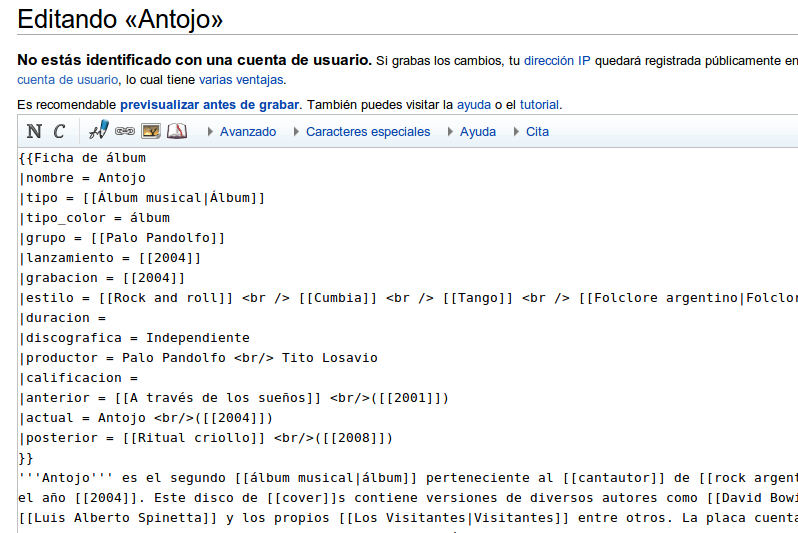
\includegraphics[width=1.0\textwidth]{fig/wiki_wysiwym}
  \caption{Editor WYSIWYM de Wikipedia}
  \label{fig:wiki_wysiwym}
\end{figure}

En la actualidad se está implantando en Wikipedia un editor WYSIWYG el cual se encuentra en fase beta y aún no soporta toda la funcionalidad del editor WYSIWYM, como por ejemplo la inserción de fórmulas matemáticas. En la figura ~\ref{fig:wiki_wysiwyg} podemos ver el aspecto de dicho editor, editando el mismo artículo que en la figura ~\ref{fig:wiki_wysiwym}.

\begin{figure}[h!]
  \centering
      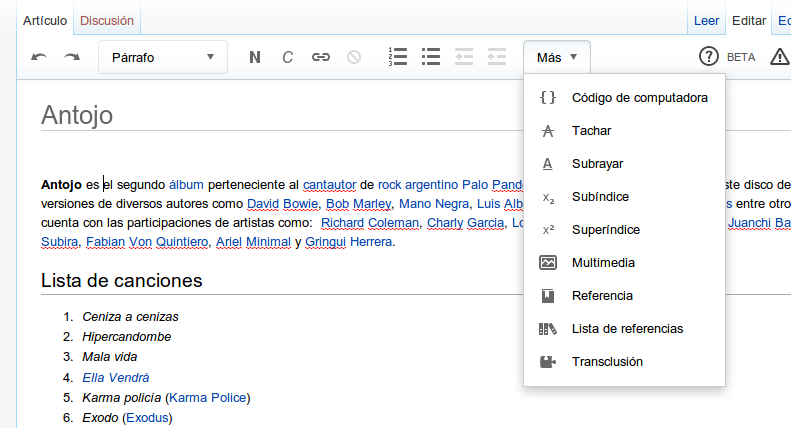
\includegraphics[width=1.0\textwidth]{fig/wiki_wysiwyg}
  \caption{Editor WYSIWYG de Wikipedia}
  \label{fig:wiki_wysiwyg}
\end{figure}

Sin embargo lo que nos interesa de Wikipedia, más que el editor en sí, es la capacidad de este para la inserción de fórmulas en {\LaTeX}~\cite{wikiform}.

MediaWiki usa un subconjunto del etiquetado AMS-LaTeX, que a su vez es un superconjunto de {\LaTeX} y presenta dos opciones para trabajar con fórmulas. La primera consiste en la generación de imágenes PNG a partir de las fórmulas usando Texvc~\cite{texvc} y la segunda que renderiza las ecuaciones mediante CSS y HTML usando MathJax~\cite{mathjax}.

Visualmente, MathJax proporciona mejores resultados. La calidad de la tipografía es muy superior y se eliminan ciertos problemas, como el diferente tamaño de las fórmulas con respecto al texto circundante o falta de alineación. Por otro lado, la herramienta javascript empleada por MathJax para interpretar las expresiones matemáticas toma más tiempo que Texvc.

Otra de las ventajas del uso de imágenes png en lugar de renderizar fórmulas con HTML y CSS es que las imágenes podrán ser almacenadas en cache, permitiendo que futuros accesos a la página sean mas rápidos.

Por otra parte, el uso de Texvc presenta el problema del tamaño de las fórmulas.
 
\subsection{Stackoverflow}
La web Stackoverflow usa un editor WYSIWYM, al estilo del que usa Wikipedia, que combina un lenguaje de etiquetado intermedio con un subconjunto del lenguaje de etiquetado HTML. Este editor posee un campo que muestra, al mismo tiempo que editamos, el resultado final del contenido que generamos. Además, tal cómo se muestra en la figura ~\ref{fig:stack_editor}, posee un menú de ayuda desplegable que permite consultarlo de forma muy cómoda mientras se escribe. Estos dos aspectos hacen que este editor sea mucho mas sencillo de usar que el editor WYSIWYM que posee Wikipedia, aunque, todo sea dicho, el editor de Wikipedia contempla funcionalidad, como el soporte de fórmulas LaTeX entre otros, que este no posee. 

\begin{figure}[h!]
  \centering
      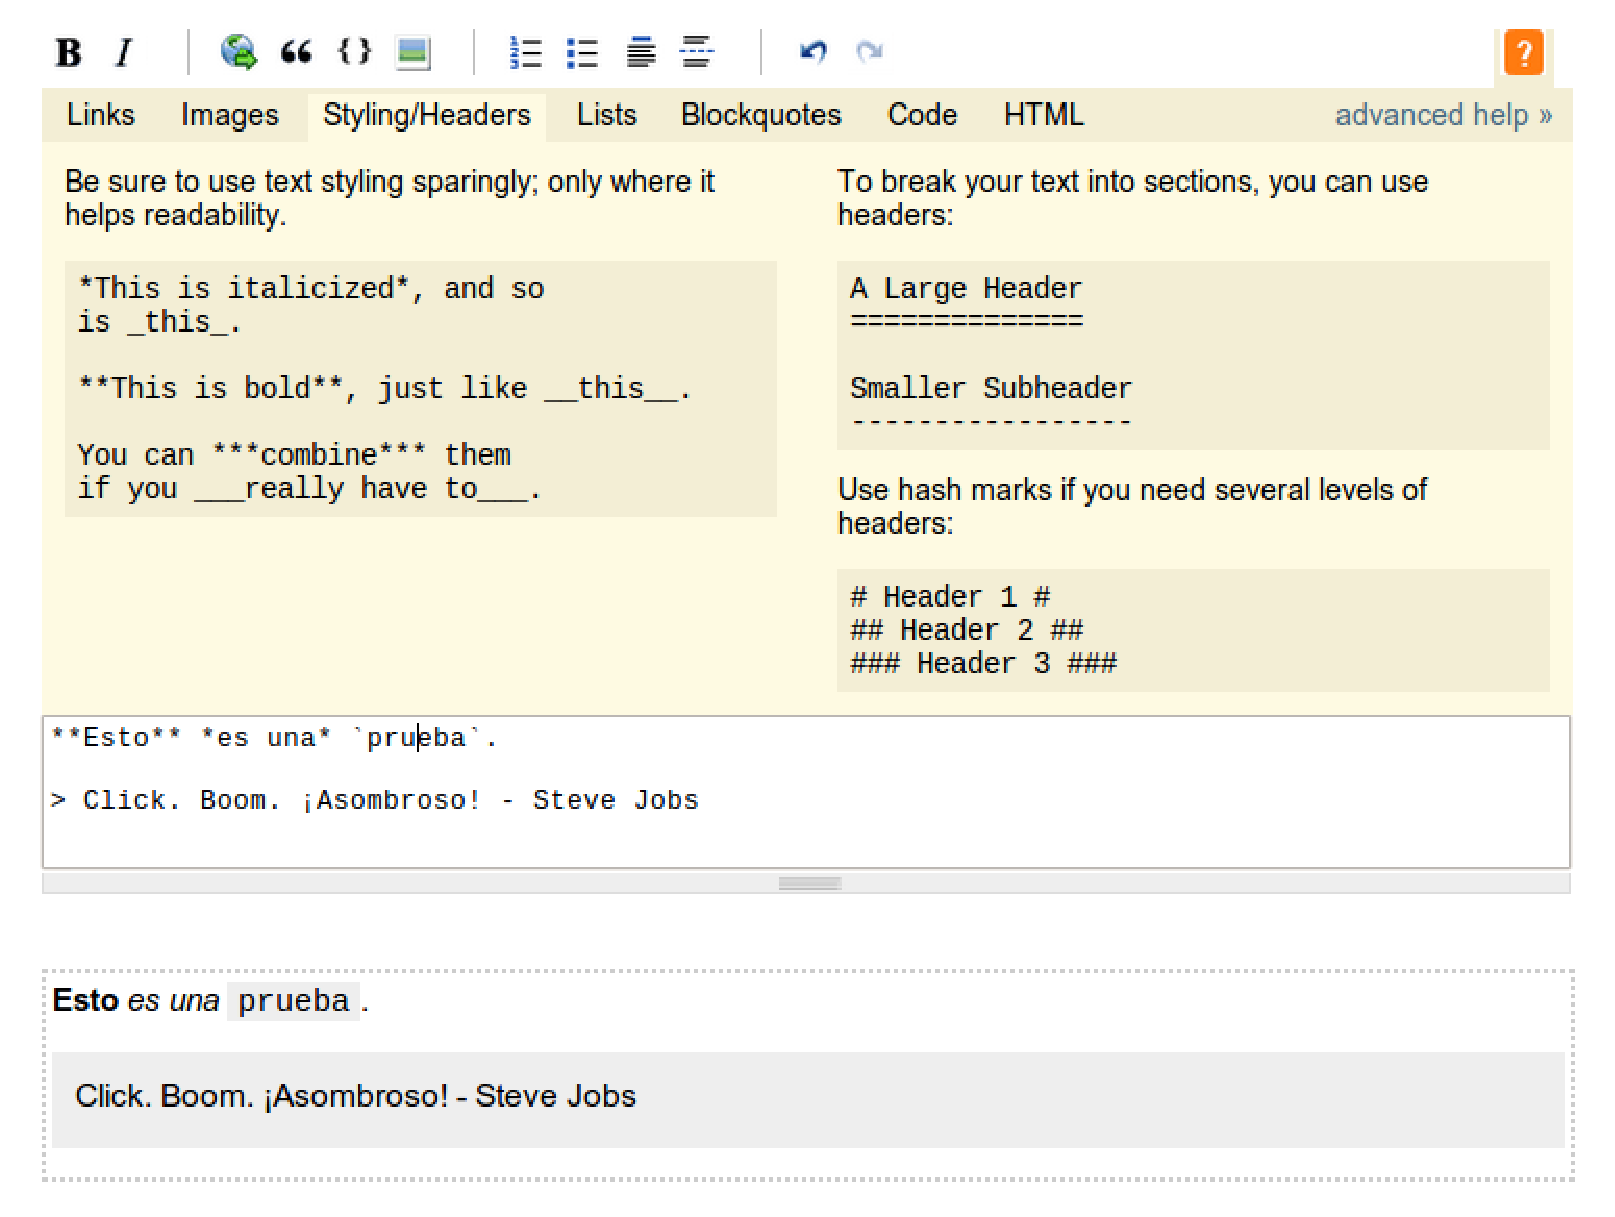
\includegraphics[width=1.0\textwidth]{fig/stack_editor}
  \caption{Editor WYSIWYM de Stackoverflow}
  \label{fig:stack_editor}
\end{figure}

\section{Renderizado de Fórmulas}
\subsection{MathJax}

MathJax, tal y como se define en su página, es un motor de visualización JavaScript para fórmulas matemáticas y de código abierto que funciona en todos los navegadores. Dicha aplicación, como ya hemos comentado previamente, nos permite renderizar las fórmulas {\LaTeX} mediante HTML y CSS.

MathJax analiza el contenido de la página buscando una fórmula en {\LaTeX} y cuando la encuentra la sustituye por un conjunto de etiquetas que compondrán la fórmula renderizada.

Esta herramienta permite dos modos de uso. La primera es enlazando directamente la aplicación a través de la Red de Distribución de Contenido (CDN) de MathJax. De esta forma MathJax siempre estará actualizado y además te ahorras su instalación en el servidor.

Sin embargo, tal cómo dijimos antes, buscamos herramientas instalables en el servidor, ya que no podemos estar sujetos a la disponibilidad de servicios de terceros. Por este motivo, si nos decantamos a usar MathJax, optaremos por la descarga e instalación de MathJax en el servidor.

\subsection{Texvc}

Texvc (Tex validator and converter) es la herramienta usada por Wikipedia para validar y generar imágenes png a partir del código en formato ams-latex. 

Dicha herramienta tiene una serie de dependencias que tendremos que satisfacer. Estas dependencias son ocaml, el lenguaje en la que está implementada y latex, dvips, gs y convert, usadas en el proceso de renderizado de la imagen de la fórmula.

A pesar de la escasa documentación disponible de esta herramienta, su extendido uso ha dado lugar a un completo FAQ con problemas de uso y soluciones para dichos problemas. El motivo por el que dicha herramienta se usa tanto es porque pertenece a la extensión math de mediawiki.

\subsection{tex2png}

Tex2png es una herramienta simple que cumple perfectamente con nuestro propósito. El autor la describe en su página~\cite{xyne:tex2png} como una herramienta para pasar fácilmente del formato {\TeX} y {\LaTeX} a PNG. Es un simple envoltorio  de \emph{latex} y \emph{divpng} que fue originalmente escrito como \emph{backend} de la web donde se aloja para insertar fácilmente fórmulas matemáticas. 

Tex2png es un script bash, por lo que su instalación consistirá únicamente en copiarlo a la carpeta desde donde lo vamos a llamar (y en la instalación de \emph{latex} y \emph{divpng}).

La documentación de esta herramienta es bastante escasa y se han encontrado algunos problemas de renderizado con algunas fórmulas. 

\section{Editores WYSIWYG}

Hay muchas personas muy inteligentes que ya han dedicado mucho tiempo a trabajar en este tema, pero esto no quiere decir que todo esté hecho. Debemos plantearnos cómo podemos mejorar estas soluciones. Obviamente, el concepto ``mejorar'' es muy difuso, puede significar que algo funcione más rápido, de una forma más novedosa o que sea más barato que el sistema original. En nuestro caso es tremendamente importante que se integre a la perfección con la plataforma SWAD y que cumpla una serie de requisitos muy concretos. En esta sección analizaremos las características de los editores WYSIWYG más usados en la Web, así como los puntos a favor y en contra de cada uno. 

También tendremos en mente las licencias bajo las que se distribuyen, pues en caso de usar parte de algún editor en nuestra solución, su licencia debe ser compatible con la licencia Affero GPL de SWAD. En la sección Apéndices podemos consultar las características generales de las distintas licencias. En caso de querer ampliar dicha información, podemos acudir a la Bibliografía.

\subsection{YUI Rich Text Editor}

Basado en la librería YUI de Yahoo y liberado bajo licencia ~\cite{BSD:bsd}, este editor sustituye el textarea estándar de HTML por un editor bastante completo. Permite dar un formato de texto enriquecido, incluyendo elementos para modificar la estructura del texto como listas, elementos para dar formato e inclusión de imágenes drag-and-drop y redimensionado de estas. Permite soporte para plugins y tiene dos modos, normal y simple, el cual tiene con un conjunto de características más reducido.

Podemos decir que se trata de un editor de alta complejidad, que se apoya en un completo Framework como es la la librería YUI de Yahoo. La Web de este editor es \url{http://yuilibrary.com/yui/docs/editor/} y allí podremos encontrar gran cantidad de información y una amplia documentación tanto de este como del Framework en el que se apoya. 

\begin{figure}[h!]
  \centering
      
\includegraphics[width=1.0\textwidth]{fig/yuie1}
  \caption{YUI Editor}
\end{figure}

\subsection{TinyMCE}

 Este popular editor WYSIWYG transforma nuestro tradicional textarea por un conjunto de elementos HTML para construir el menú de formato, esta herramienta es muy usada por diversos CMS (Content Management System ) Open Source, es muy fácil de integrar, permite la personalización de botones en la barra de herramientas y tiene opciones para configurar el menú de formato limitando el número de botones que aparecen. Como ventaja comentar que se distribuye bajo la licencia de código abierto LGPL~\cite{LGPL:lgpl} y que es fácil de integrar y personalizar. Para probar este editor o ampliar esta información se recomienda consultar la web \url{http://www.tinymce.com/}.

\begin{figure}[h!]
  \centering
      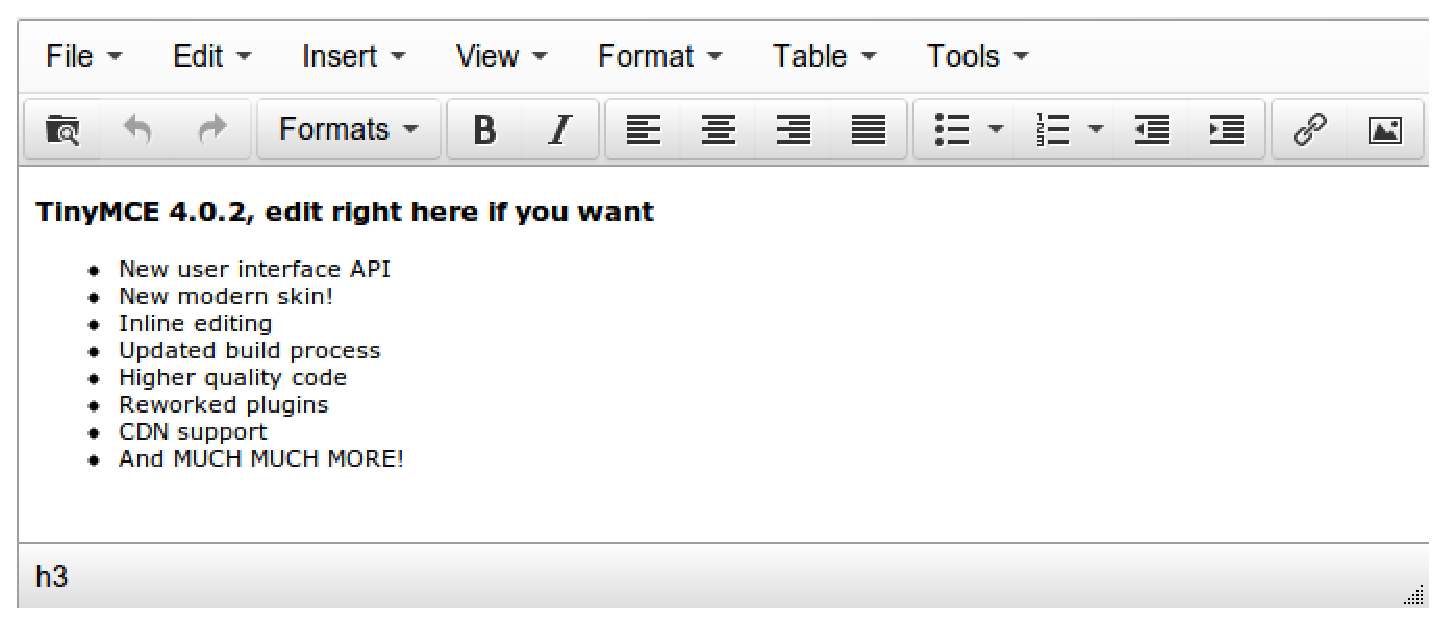
\includegraphics[width=1.0\textwidth]{fig/tmce1}
  \caption{Tinymce Editor}
\end{figure}

\subsection{NicEdit}

Este ligero editor WYSIWYG, distribuido bajo Licencia MIT~\cite{MITL:mitl}, se caracteriza por su flexibilidad, sencillez y capacidad de personalización. Permite transformar cualquier elemento div o textarea en un editor de texto enriquecido. Se trata de un editor simple pero efectivo. Al contrario que otros editores, no viene con distintos skins o plugins para ampliar su funcionalidad, ni tiene soporte nativo para fórmulas. 

Permite limitar la funcionalidad mediante la selección de los elementos que aparecerán en la barra de herramientas y, a excepción del editor de fórmulas, implementa toda la funcionalidad que requerirá nuestro editor. De fácil instalación y uso es una opción muy a tener en cuenta. La integración en la página es muy simple y puede llevarse a cabo con un par de líneas de código. Para más información visitar su web: \url{http://nicedit.com/}.


\begin{figure}[h!]
  \centering
      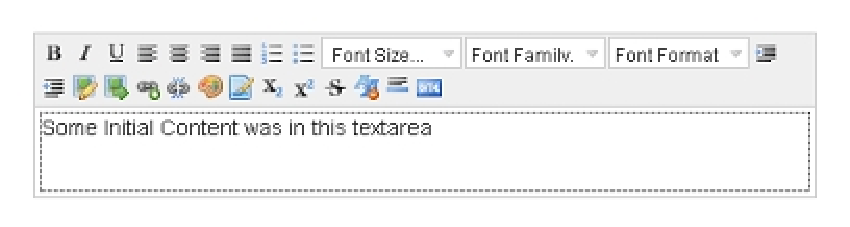
\includegraphics[width=1.0\textwidth]{fig/nice1}
  \caption{NicEdit Editor}
\end{figure}

\subsection{CKeditor}

Este editor WYSIWYG es muy potente y estable a la vez que flexible. Ampliamente usado, cuenta con una trayectoria de 10 años en el mercado. Además genera código XHTML de calidad, permitiendo su edición y parsea el contenido para que este no afecte a la página que contiene al editor. Permite el uso de plugins desarrollados por terceros y con estos amplia notablemente la funcionalidad del editor. La apariencia está muy cuidada y hay disponibles varios skins que podemos usar. Distribuido bajo las licencias de código abierto GPL~\cite{GPL:gpl}, LGPL~\cite{LGPL:lgpl} y MPL~\cite{MPL:mpl}.

Presenta la ventaja de tener soporte para fórmulas mediante plugins. Los plugins con esta finalidad disponibles son dos: Math Editor y WIRIS math \& science editor. El primero funcionaba correctamente en pruebas online, pero al probarlo en nuestro servidor no hemos conseguido que funcione en ningún navegador, muy probablemente por imcopatibilidades con la versión de CKEditor. El segundo plugin cumple con su cometido, aunque desde mi punto de vista es demasiado complejo. Tras seleccionar la opción de fórmulas, tal y como se muestra en la Figura ~\ref{fig:ckmath}, se abre una nueva ventana que contiene un completo editor donde podemos escribir nuestra fórmula. Una vez confirmada la operación se inserta en nuestro editor la imagen correspondiente a la fórmula escrita. Pese a estos pequeños fallos en los plugins, que recordemos han sido desarrollados por terceros, el editor en sí es muy completo y permite entre otras cosas la edición de texto en linea al hacer click sobre este. 

Para más información podemos consultar su web: \url{http://ckeditor.com/}

\begin{figure}[h!]
  \centering
      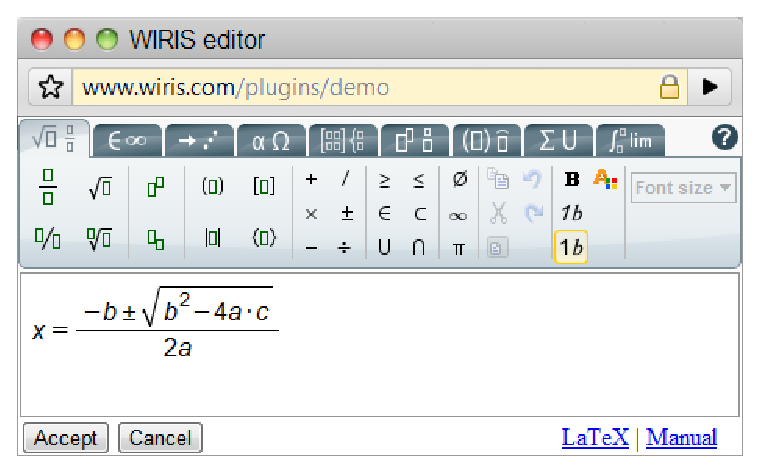
\includegraphics[width=1.0\textwidth]{fig/cke3}
  \caption{Plugin WIRIS para CKEditor}
  \label{fig:ckmath}
\end{figure}

\begin{figure}[h!]
  \centering
      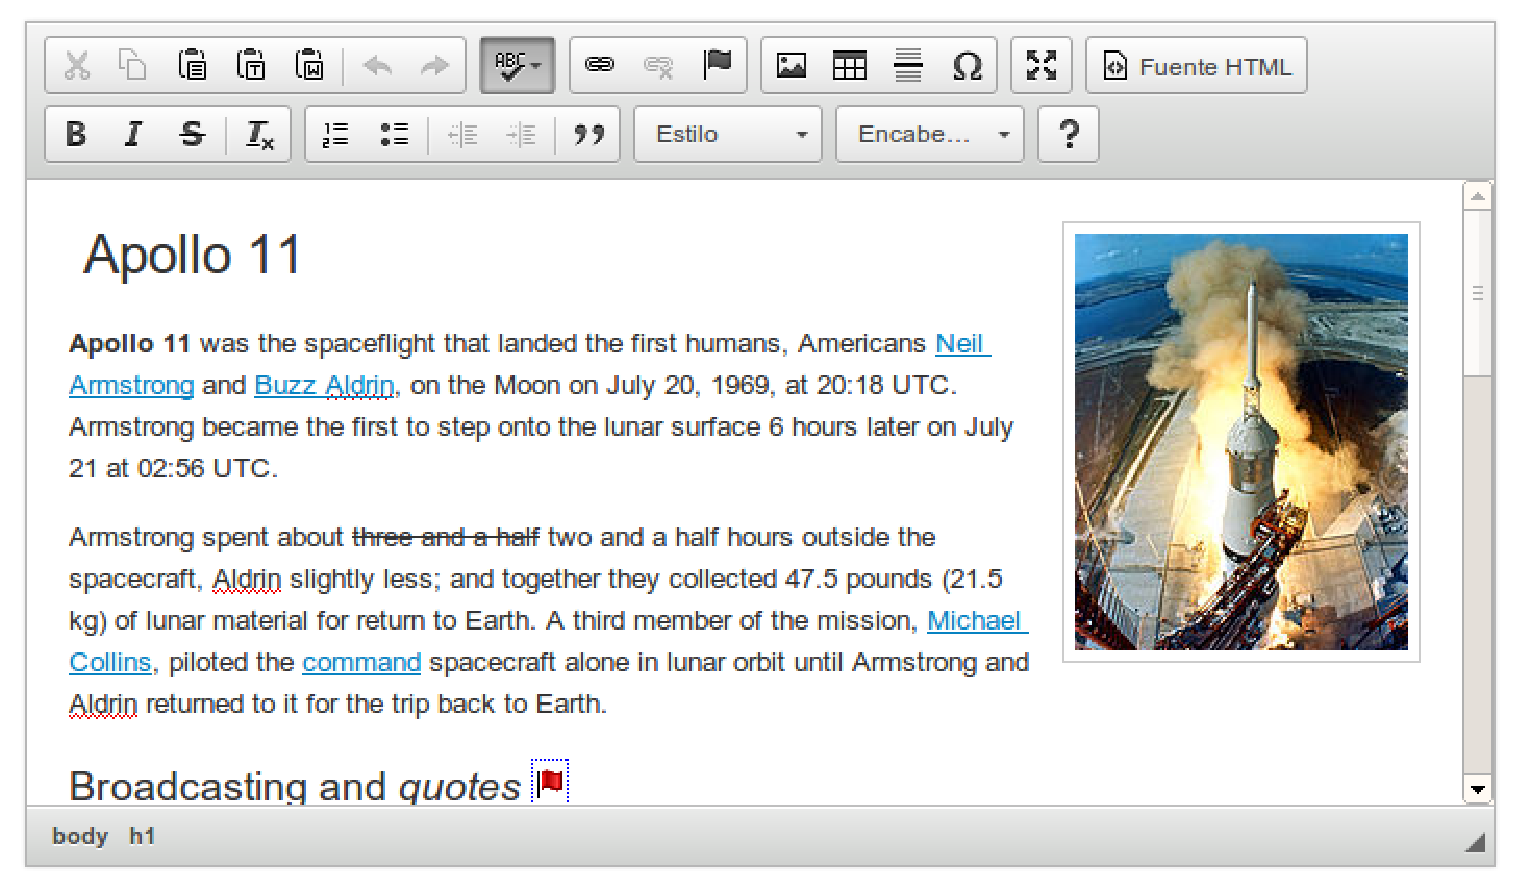
\includegraphics[width=1.0\textwidth]{fig/cke1}
  \caption{CKEditor}
\end{figure}

\subsection{openWYSIWYG}
\url{http://www.openwebware.com}
Este sencillo editor, distribuido bajo licencia de código abierto LGPL~\cite{LGPL:lgpl}, se presenta como el editor ideal para mejorar tu CMS. Como los anteriores remplaza textarea por un editor de texto. Parece ser que en la actualidad se encuentra obsoleto y presenta incompatibilidades con los navegadores actuales. Su web es \url{http://www.openwebware.com}.


\begin{figure}[h!]
  \centering
      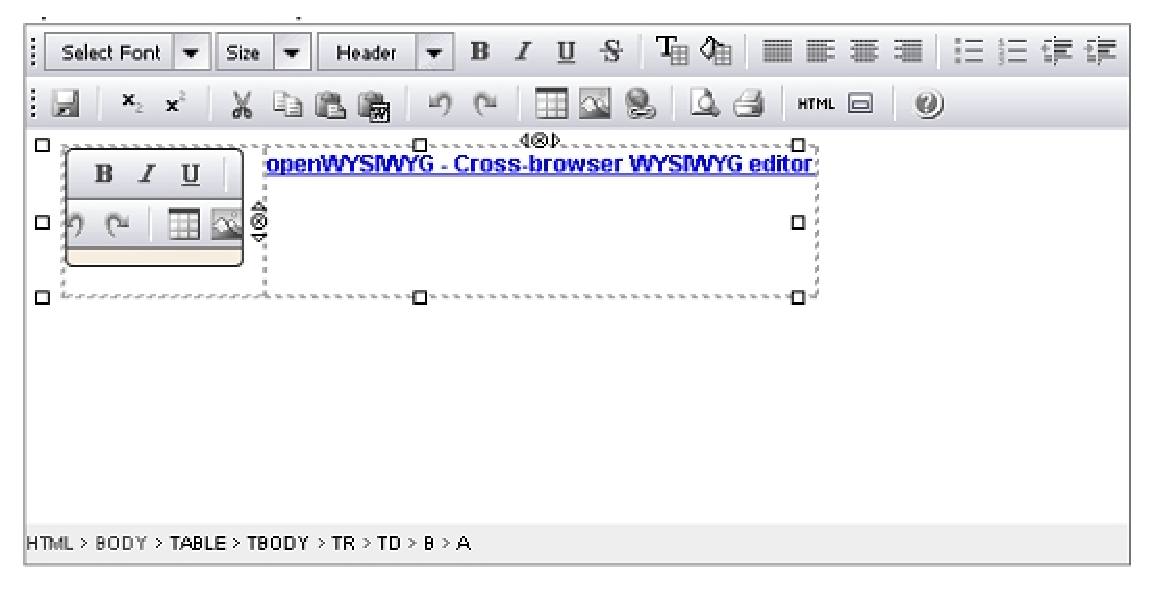
\includegraphics[width=1.0\textwidth]{fig/opene1}
  \caption{openWYSIWYG Editor}
\end{figure}


\section{Conclusiones del Análisis}

En este capítulo hemos analizado y reflexionado acerca de diversas plataformas y herramientas de la Web. A continuación veremos cuales de estas se ajustan más a nuestros objetivos, teniendo siempre en mente los requisitos de nuestro editor y buscando una solución sencilla y de calidad.

En lo referente a los editores descartamos el uso de \emph{openWYSIWYG} debido a los problemas de compatibilidad con los distintos navegadores que ha presentado, ya que parece ser que dicho editor se encuentra obsoleto.

Por otra parte hay algunos editores que soportan de forma nativa (o con el uso de plugins) el uso de fórmulas. Este es el caso de \emph{CKEditor} y \emph{YUI Rich Text Editor}.

\emph{CKEditor} es un proyecto maduro con 10 años en el mercado. Esta madurez se nota en todos los aspectos. El acabado de CKEditor es impecable, no tanto lo es el de sus plugins, desarrollados por terceros. A pesar de esto CKEditor es una opción muy a tener en cuenta. El problema que presenta, sin duda, es que esta complejidad de la que hace gala puede convertirse en un problema a la hora de estudiar y modificar su código fuente para adaptarlo a nuestras necesidades. Comentar también la posibilidad de usar cualquiera de las licencias ~\cite{GPL:gpl}, LGPL~\cite{LGPL:lgpl} y MPL~\cite{MPL:mpl}, lo que nos aporta gran libertad.
      
\emph{TinyMCE} supone una alternativa de calidad a \emph{CKEditor}. A diferencia de este último \emph{TinyMCE} se distribuye solo bajo licencia LGPL, lo que algunos casos podría ser una restricción. Sin embargo, en este caso concreto, no es importante ya que SWAD se encuentra liberado bajo una licencia AGPLv3 y no presentaría incompatibilidades con la licencia LGPL del editor. 

\emph{YUI Rich Text Editor} presenta una potente alternativa, con el respaldo de una gran empresa como es YAHOO. Como ya comentamos antes, se basa en el framework YUI (Yahoo User Interface), una serie de bibliotecas escritas en JavaScript para la construcción de aplicaciones de Internet enriquecidas (RIA) y liberadas bajo licencia BSD por parte de la compañía Yahoo. Sin embargo, para nuestro editor, evitaremos el uso de frameworks y nos basaremos en algún editor ``standalone''.

\emph{NicEdit} es una solución simple, aunque carece de soporte nativo para fórmulas, funcionalidad que tendríamos que ampliar con alguna otra herramienta, como puede ser MathJax o Texvc. A excepción de esto último, NicEdit implementa toda la funcionalidad necesaria por nuestro editor.

Al parecer, las mejores opciones para nuestro editor son NicEdit y CKEditor. CKEditor es mas pesado que NicEdit aunque mucho mas completo y con muchos plugins desarrollados por terceros. Dada la simplicidad del problema que nos ocupa, la ligereza de NicEdit es un gran punto a su favor, haciéndose innecesarios la gran mayoría de los plugins que tiene CKEditor. Por otra parte, el plugin WIRIS de fórmulas para CKEditor también está disponible para NicEdit. 

El problema de modificar un editor ya existente es que requiere una compleja labor de estudio de su código fuente para poder eliminar aquella funcionalidad que no necesitamos y añadir la funcionalidad de la que carece, así como adaptarlo a nuestros requisitos.  

Tras un completo análisis del código fuente de los editores se ha decidido implementar nosotros mismos el editor WYSIWYG, evitando el uso de cualquier Framework y desarrollando la solución lo más simple posible, cumpliendo cada uno de nuestros requisitos. Aunque no tomemos código fuente de ninguno de los editores anteriormente comentados, nos inspiraremos en NicEdit, el ligero editor que más se ajustaba a nuestras necesidades.



